% The twelve steps of the design and the feedback loop (manuscript Section 3.3); gap letters refer to Section 3.1.
% Build: pdflatex fig10_steps.tex; pdftoppm -r 220 -png -singlefile fig10_steps.pdf fig10_steps
\documentclass[tikz,border=2pt]{standalone}
\usepackage{times}
\usetikzlibrary{positioning,arrows.meta,calc}
\begin{document}
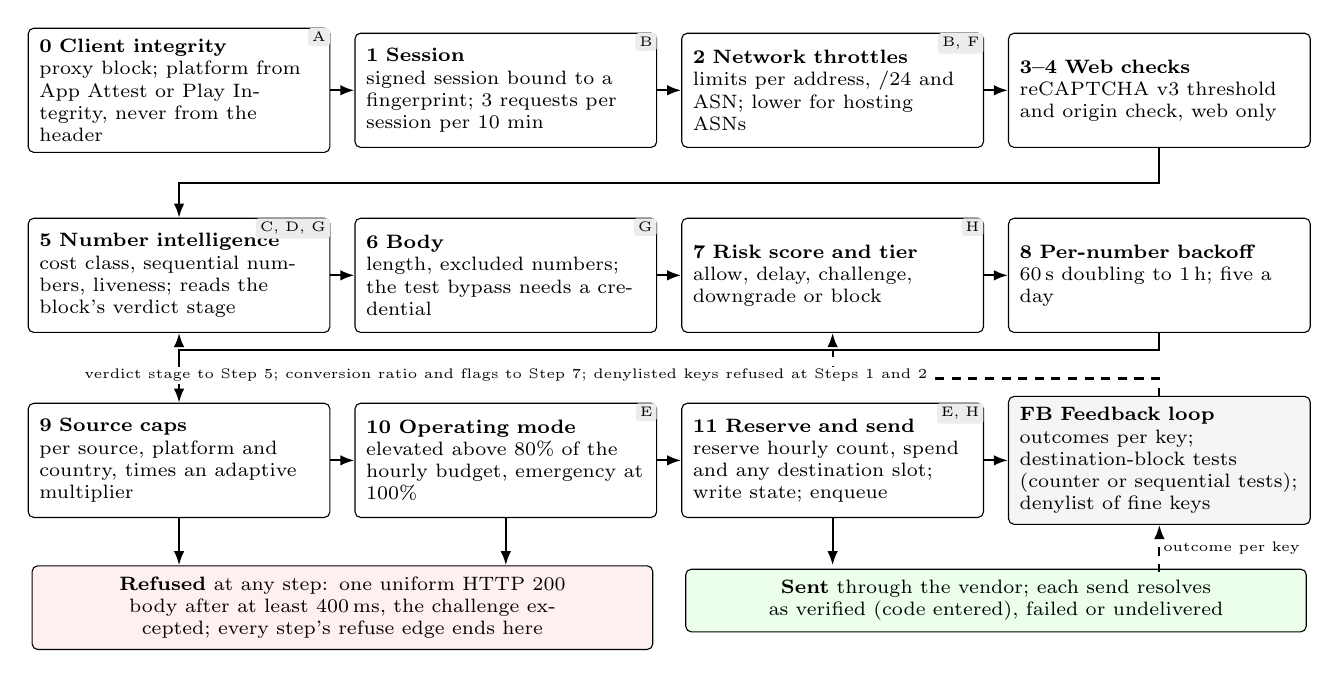
\begin{tikzpicture}[
  sbox/.style={draw, rounded corners=2pt, align=left, text width=3.55cm, minimum height=1.45cm, font=\scriptsize, inner sep=4pt, fill=white},
  num/.style={font=\scriptsize\bfseries},
  gapbadge/.style={font=\tiny, fill=gray!15, inner sep=1.5pt, rounded corners=1pt, anchor=north east},
  arr/.style={-{Latex[length=1.8mm]}, thick},
  ret/.style={-{Latex[length=1.8mm]}, thick, dashed},
  sink/.style={draw, rounded corners=2pt, align=center, font=\scriptsize, fill=red!6, inner sep=4pt},
  lab/.style={font=\tiny, fill=white, inner sep=1pt}
]
\def\dx{4.15cm}\def\dy{-2.35cm}
% row 1
\node[sbox] (s0) at (0,0) {\textbf{0 Client integrity}\\proxy block; platform from App Attest or Play Integrity, never from the header};
\node[sbox] (s1) at (\dx,0) {\textbf{1 Session}\\signed session bound to a fingerprint; 3 requests per session per 10 min};
\node[sbox] (s2) at (2*\dx,0) {\textbf{2 Network throttles}\\limits per address, /24 and ASN; lower for hosting ASNs};
\node[sbox] (s3) at (3*\dx,0) {\textbf{3--4 Web checks}\\reCAPTCHA v3 threshold and origin check, web only};
% row 2
\node[sbox] (s5) at (0,\dy) {\textbf{5 Number intelligence}\\cost class, sequential numbers, liveness; reads the block's verdict stage};
\node[sbox] (s6) at (\dx,\dy) {\textbf{6 Body}\\length, excluded numbers; the test bypass needs a credential};
\node[sbox] (s7) at (2*\dx,\dy) {\textbf{7 Risk score and tier}\\allow, delay, challenge, downgrade or block};
\node[sbox] (s8) at (3*\dx,\dy) {\textbf{8 Per-number backoff}\\60\,s doubling to 1\,h; five a day};
% row 3
\node[sbox] (s9) at (0,2*\dy) {\textbf{9 Source caps}\\per source, platform and country, times an adaptive multiplier};
\node[sbox] (s10) at (\dx,2*\dy) {\textbf{10 Operating mode}\\elevated above 80\% of the hourly budget, emergency at 100\%};
\node[sbox] (s11) at (2*\dx,2*\dy) {\textbf{11 Reserve and send}\\reserve hourly count, spend and any destination slot; write state; enqueue};
\node[sbox, fill=gray!8] (fb) at (3*\dx,2*\dy) {\textbf{FB Feedback loop}\\outcomes per key; destination-block tests (counter or sequential tests); denylist of fine keys};
% gap badges
\node[gapbadge] at (s0.north east) {A};
\node[gapbadge] at (s1.north east) {B};
\node[gapbadge] at (s2.north east) {B, F};
\node[gapbadge] at (s5.north east) {C, D, G};
\node[gapbadge] at (s6.north east) {G};
\node[gapbadge] at (s7.north east) {H};
\node[gapbadge] at (s10.north east) {E};
\node[gapbadge] at (s11.north east) {E, H};
% flow
\draw[arr] (s0) -- (s1); \draw[arr] (s1) -- (s2); \draw[arr] (s2) -- (s3);
\draw[arr] (s3.south) -- ++(0,-0.45) -| (s5.north);
\draw[arr] (s5) -- (s6); \draw[arr] (s6) -- (s7); \draw[arr] (s7) -- (s8);
\draw[arr] (s8.south) -- ++(0,-0.22) -| (s9.north);
\draw[arr] (s9) -- (s10); \draw[arr] (s10) -- (s11);
\draw[arr] (s11) -- (fb);
% send and outcomes
\node[sink, fill=green!8, text width=7.6cm, below=0.6cm of $(s11.south)!0.5!(fb.south)$] (send) {\textbf{Sent} through the vendor; each send resolves as verified (code entered), failed or undelivered};
\draw[arr] (s11.south) -- ($(s11.south)+(0,-0.6)$);
\draw[ret] ($(fb.south)+(0,-0.6)$) -- (fb.south) node[lab, midway, right]{outcome per key};
% feedback into earlier steps
\draw[ret] (fb.north) -- ++(0,0.22) -| (s7.south);
\draw[ret] ($(fb.north)+(0,0.22)$) -| (s5.south);
\node[lab, anchor=north] at ($(s6.south)+(0,-0.42)$) {verdict stage to Step 5; conversion ratio and flags to Step 7; denylisted keys refused at Steps 1 and 2};
% refusals
\node[sink, text width=7.6cm, below=0.6cm of $(s9.south)!0.5!(s10.south)$] (refuse) {\textbf{Refused} at any step: one uniform HTTP 200 body after at least 400\,ms, the challenge excepted; every step's refuse edge ends here};
\draw[arr] (s9.south) -- ($(s9.south)+(0,-0.6)$);
\draw[arr] (s10.south) -- ($(s10.south)+(0,-0.6)$);
\end{tikzpicture}
\end{document}
